\documentclass[tikz,border=2mm]{standalone}
\usetikzlibrary{shadings,calc}
\begin{document}
	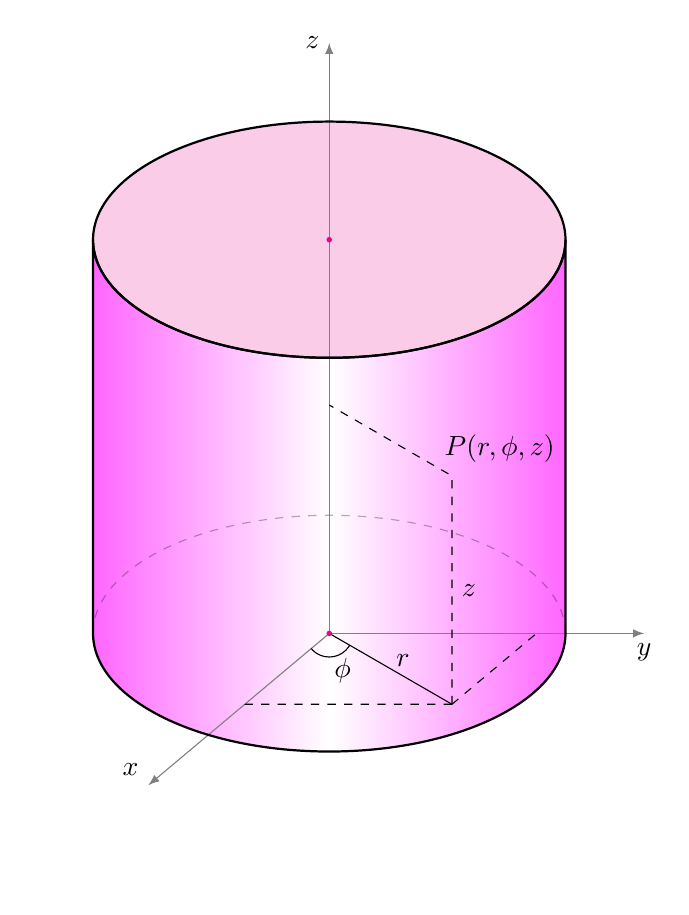
\begin{tikzpicture}
		\def\a{3} % bán trục lớn = bán kính trụ
		\def\b{1.5} % bán trục nhỏ
		\def\h{5} % chiều cao trụ
		% tạo hiệu ứng 3D: cho màu cánh sen nhạt
		% tạo vết nhạt dần từ 2 bên, đến màu trắng ở giữa (thư viện shadings)
		\fill[left color=magenta!60,right color=magenta!60,middle color=white]
		(\a,0)--(\a,\h) arc(0:-180:{\a} and {\b})--
		(-\a,0) arc(180:360:{\a} and {\b})--cycle;
		\draw[dashed,opacity=.3] (\a,0) arc(0:180:{\a} and {\b});
		\fill[magenta!20!white] (\a,\h) arc(0:360:{\a} and {\b});
		\draw[gray,-latex] (0,0)--(\a,0)--([turn]0:1cm)
		node[below,black]{$y$};
		\draw[gray,-latex] (0,0)--(0,\h)--([turn]0:2.5cm)
		node[left,black] {$z$};
		\def\gocX{-140}
		\draw[gray,-latex] (0,0)--(\gocX:\a)
		node[above left,black] {$x$};
		\def\gocQ{-30}
		\def\r{1.8}
		\draw (0,0)--(\gocQ:\r) coordinate (Q)
		node[above,pos=.6]{$r$};
		\draw[dashed] (Q)--++(90:2.9) coordinate (P)
		node[right,midway]{$z$}
		node[shift={(30:7mm)}]{$P(r,\phi,z)$}--($(0,0)+(P)-(Q)$) ;
		\begin{scope}
			\clip (\gocX:\a+2)--(0,0)--(\a,0) arc(0:\gocX:\a)--cycle;
			\draw[dashed](Q)--+(180:\a) (Q)--+(180+\gocX:\b);
		\end{scope}
		\fill[magenta] (0,0) circle(1pt) (0,\h) circle(1pt);
		\draw[thick] (\a,0)--(\a,\h) arc(0:-180:{\a} and {\b})--
		(-\a,\h)--(-\a,0) arc(180:360:{\a} and {\b})--(\a,0)--cycle;
		\draw[thick] (\a,\h) arc(0:360:{\a} and {\b});
		\clip (\gocX:\a+2)--(0,0)--(Q)--cycle;
		\draw (0,0) circle(3mm) (.5*\gocX:5mm) node{$\phi$};
	\end{tikzpicture}
\end{document}